\section{Functions}
The purpose of these exercises is to round up all the knowledge learned from the former workshops and use it as building blocks in functions. It should also teach the students how to call a function, and what happens when calling it in a program. Firstly, you should walk the student through this introduction.

\subsection{Introduction}
A function is a sequence of instructions that you save such that you can reuse them. An example could be that you need to write a text message to your friend Eric. The instructions could look like:

Function text friend()
\begin{itemize}
    \item[-] Open text app
    \item[-] Click on Eric
    \item[-] Write "hello"
    \item[-] Click on send
\end{itemize}
These instructions could be saved in your "program", and you could then reuse them to send a text to Eric again. If you, however, wanted to text your friend Anna, these specific instructions would not work. This is where our \textbf{arguments} come to help. Arguments are interchangeable variables integrated in the program. So your send message instructions could be updated with an argument for it to be usable for all your friends:

Function text friend(\textbf{name})
\begin{itemize}
    \item[-] Open text app
    \item[-] Click on \textbf{name}
    \item[-] Write "hello"
    \item[-] Click on send
\end{itemize}
Now, when you need to use the function to text Anna, you replace the argument \textbf{name} with "Anna".

When you create a function, it needs a name, maybe some arguments, and then inside the instructions. 

We also have a coded example. This code is a function for the game "Fizz Buzz", where we use two arguments: two numbers. The function counts from 0 to infinity, and whenever the counter is divisible by the fizz argument, it says "Fizz", whenever the counter is divisible by the buzz argument, it says "Buzz", and likewise, if the counter is divisible by both the fizz and buzz argument, it says "Fizz Buzz". Lets walk through it together.

\subsection{Exercises}
The student is given the building blocks needed for a specific function, and should build it themself. The building blocks are LEGO Duplos with instructions printed on them.

\subsubsection{Multiplication function - easy}
The first exercise is to make a function that multiplies two numbers without using the multiplication operator.
\begin{figure}
    \centering
    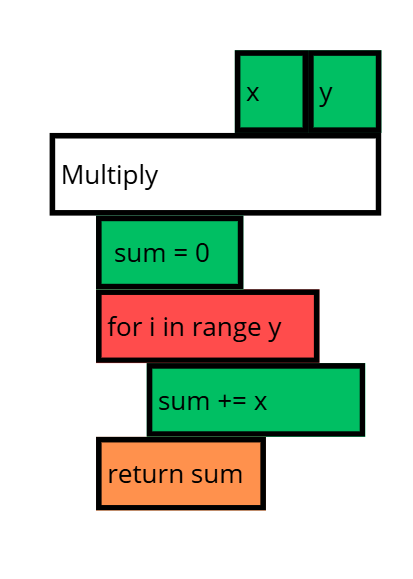
\includegraphics[width=0.5\linewidth]{Billeder/Multiplication function.png}
\end{figure}

\subsubsection{Power function - hard}

\subsection{\texttt{print} vs \texttt{return}}
This section is to introduce the distinction between print and return. This is not necessarily computational thinking, but important when learning programming in Python and could come up when learning about functions.

Imagine you have a coffee machine as your function. You press a button and then something happens. With \texttt{print}, the machine just says something out loud:

\texttt{\\
\ \ def make\_coffee():\\
\ \ \ \ \ \ print("Here is your coffee!")\\
}

When you call your function, the result on the screen is just \texttt{Here is your coffee!}, but there's nothing to store or reuse. You can't give the coffee to someone else or save it for later; it's just a message. Now compare that to using \texttt{return}:

\hspace*{2em} \texttt{\\
\ \ def make\_coffee():\\
\ \ \ \ \ \ return "A cup of coffee"\\
}

Now when you call your function, it makes a cup of coffee and gives it to you. You can then save your cup of coffee in a variable:

\texttt{\\
\ \ my\_coffee = make\_coffee()\\
}

And this time, the coffee is actually saved in the variable \texttt{my\_coffee}, so you can use it later, just like having a real cup in your hand.